%
%
%
%
%\chapter{Le programme cosmologique de NIKA2}
%\label{se:cosmo_NIKA2}

%----------------------------------------------------------------------------------------
%
%
%
%
%                COSMO HAUTE-RESOLUTION
%                 
%
%
%
%----------------------------------------------------------------------------------------
\section{Cosmologie CMB à haute résolution angulaire}
\label{se:CMB-HR}

NIKA2 s'inscrit dans l'effort expérimental dans le domaine du CMB. 
Après le succès des expériences mesurant les grandes échelles
angulaires~\citep[BICEP2 et Keck Array][]{BK2018} et celles à
résolution angulaire de 1 à 4', telles SPT-SZ et
SPTpol~\citep{deHaan2016, SPTpol2019}, ACT et
ACTpol~\citep{ACTpol2017, ACTpol2018} ou
POLARBEAR~\citep{Polarbear2017}, les expériences CMB au sol se
développent tout azimut, avec BICEP3~\citep{BICEP3_2018},
\emph{Advanced ACTpol}~\citep{AdvACT2018}, SPT-3G~\citep{SPT3G_2018}
ou le \emph{Simons Array}~\citep{SA_2016}. Pour la future génération
d'expériences, les efforts se rassemblent dans des
meta-collaborations multi-sites, telles
CMB-S4~\footnote{\url{http://CMB-S4.org}}, dont les précurseurs, tel
le \emph{Simons Observatory}~\citep{SO2019} sont
en cours de construction. L'objectif étant de combiner très haute
sensibilité à la polarisation pour espérer détecter le mode B
primordial qui signe la fin de l'inflation et résolution angulaire de
l'ordre de la minute d'arc pour assurer une bonne mesure des
anisotropies secondaires, en particulier l'effet de lentille
gravitationnelle sur le CMB, qui a aussi un impact sur le mode B
primordial, et l'effet SZ pour sonder la matière baryonique à haut
redshift. En particulier, le \emph{Simons Observatory}, dont la
première lumière est prévue en 2021, détectera dix fois plus d'amas
de galaxies que \emph{Planck} et exploitera aussi bien l'abondance des
amas que les propriétés statistiques de la carte de paramètre de
Compton pour dériver des contraintes compétitives sur la cosmologie,
par exemple dans le secteur des neutrinos.  
%Les exigences observationnelles pour la mesure du
%SZ étant les memes que celles du CMB lensing, la cosmologie avec le SZ
%est aussi en tres fort développement.
De plus, avec la perspective d'exploiter l'effet SZ cinétique pour
mesurer les propriété thermodynamique des amas, les effets baryoniques
non-thermiques, la dispersion des vitesses et le début du processus de
réionisation, une nouvelle voie très prometteuse
s'ouvre~\citep{SO2019}. La cosmologie avec le SZ est donc un objectif
scientifique prioritaire des futures expériences CMB.

En parallèle, d'importants efforts instrumentaux sont déployés dans le
domaine CMB/millimétrique pour atteindre des résolutions angulaires en
deçà de la minute d'arc. NIKA2 participe de cet effort. D'autres
expériences à haute résolution angulaire dans le domaine
millimétrique, à fort impact sur la physique des amas
de galaxie via l'exploitation de l'effet SZ, sont actuellement en
fonctionnement ou en projet. Parmi celles-ci, on peut citer l'imageur
MUSTANG-2, installé au \emph{Green Bank telescope} de 100 mètres,
ouvert à la communauté depuis 2018, capable de carthographier un champ
de vue de 4.35’ à 90\,GHz avec une résolution angulaire de
9''~\citep{Dicker2014_MUSTANG2, Stanchfield2016_MUSTANG2}. En
particulier, l'utilité de MUSTANG-2 pour mesurer le profil de
pression des amas de galaxie via l'effet tSZ à été récemment
démontrée~\citep{Romero2019_SZ}.
Autre exemple, l'observatoire interférométrique \emph{Atacama Large
  Millimeter/Submillimeter Array} (ALMA), qui inclut trois réseaux
d'antennes de sept à douze mètres de diamètre, peut imager un champ de
vue jusqu'à environ 1.5' à une résolution de quelques seconde d'arc
dans la gamme de fréquence 84 à 950\,GHz~\citep{ALMA2008, Iguchi2009}.
Dans le domaine du SZ, ALMA a récemment fourni une cartographie à une
résolution de 3.5'' d'un choc dans un amas en
collision~\citep{Basu2016}. La future génération d'expériences
millimétriques/sub-millimétriques haute-résolution est d'ores et déjà en
construction. Ces projets incluent \emph{TolTEC}, au
\emph{Large Millimeter-wave Telescope} de 50 mètres de diamètre,
capable d'imager un champ de vue de 4' à une résolution de 10 à 5''
dans trois bandes de fréquence centrées à 150, 220 et
280\,GHz~\citet{bryan_optical_2018}; CONCERTO, un spectromètre qui
sera installé au télescope de 12-m de l'\emph{Atacama Pathfinder
  Experiment} (APEX) et couvrira la gamme de
fréquence de 125 à 360\,GHz avec un champ de vue d'environ 15' et une
résolution angulaire maximale de 20''~\citep{Lagache2018}; 
CCAT-prime est un télescope de 6-m de diamètre dont l'exploitation
devrait commencer en 2021 sur le site de \emph{Cerro Chajnantor}, pour
ouvrir la voie à la construction d'un télescope de 25-m (CCAT) sur ce
site exceptionnel~\citep{Stacey2018}; Il accueillera l'imageur
\emph{Prime-Cam}, dont les observations dans une gamme de fréquence où
le signal SZ est positif devrait permettre de séparer les contributions
tSZ, kSZ et rSZ dans les futurs relevés d'amas de
galaxies via l'effet SZ~\citep{Mittal2018}. On se reportera à
\citet{Tony2019} pour une revue récente de l'effet SZ à haute
résolution.

Pour la cosmologie, l'objectif des expériences millimétriques à très
haute résolution angulaire est double. Il s'agit d'une part d'obtenir
des cartographies de plus en plus profondes
de l'univers distant en reculant la limite de confusion, avec pour
objectif de contraindre l'évolution cosmique de la formation d'étoile
et les scenarii de la réionisation de l'Univers~\citep{Mancuso2016,
  Bethermin2017_simu}. D'autre part, ces expériences permettent de
sonder la structure interne des amas de galaxie et de contraindre
l'évolution de leur propriétés avec le redshift afin d'améliorer leur
exploitation en cosmologie, comme discuté à la
Sect.~\ref{se:cosmo_tensions}. Ces deux approches cosmologiques
constituent des objectifs prioritaires de NIKA2,
mobilisant chacun un large programme d'observation en temps
garanti. Mon projet de recherche dans NIKA2 s'inscrit dans le grand
programme dédié à la cosmologie avec les amas de galaxie, dont je suis
\emph{Principal Investigator} aux côtés de Frédéric Mayet. 



%----------------------------------------------------------------------------------------
%
%
%
%
%
%                 DESCRIPTION LP-SZ
%
%
%
%----------------------------------------------------------------------------------------
\section{Le grand programme d'observation d'amas de galaxies}
\label{se:LP-SZ}

La cosmologie avec les amas de galaxies est actuellement limitée par
la précision avec laquelle la masse des amas peut être déterminée, en
particulier à des redshifts $\gtrsim 0.4$, comme discuté à la
Sect.~\ref{se:cosmo_tensions}. Ainsi, une étude détaillée des propriétés
thermodynamiques du milieu intra-amas et de la morphologie des amas de
galaxies dans un large échantillon incluant des amas distants
($z\gtrsim 0.7$) permettrait d'améliorer les résultats cosmologiques se
fondant sur cette sonde. L'expérience NIKA2, décrite au
chapitre\,\ref{chap:nika2iram} et dont les performances ont
été détaillées aux chapitres\,\ref{chap:calib_perf} et
\,\ref{chap:nika2_resume}, nous offre une opportunité unique pour mener
une telle étude, via une cartographie haute-résolution de l'effet SZ
d'un échantillon d'amas couvrant une large gamme de redshifts. C'est
là l'objectif du grand programme SZ~\footnote{site web :
  \url{http://lpsc.in2p3.fr/NIKA2LPSZ/}} (LP-SZ) de NIKA2.


\subsection{L'échantillon d'amas}
Le LP-SZ est l'un des cinq grands programmes sélectionnés par le
consortium NIKA2-IRAM et à ce titre, bénéficie de 300 heures
d'observation (\emph{Guaranteed Time}) avec l'expérience NIKA2 au
télescope de 30-m de l'IRAM.

Le LP-SZ cible un échantillon représentatif de 50 amas de galaxies à
redshifts intermédiaires et à hauts redschifts ($0.5 < z < 0.9$),
sélectionnés dans les catalogues d'amas de \emph{Planck} et ACT. La
distribution spatiale, ainsi que la distribution en masse et redshift
des amas de l'échantillon est présentée à la Fig.~\ref{fig:LP-SZ}.
%
\begin{figure}
  \centering
  \includegraphics[width=0.49\textwidth]{Figures/NIKA2-SZ/Figure_LPSZ_dust_map_FR.jpg}
  \hspace{4mm}
  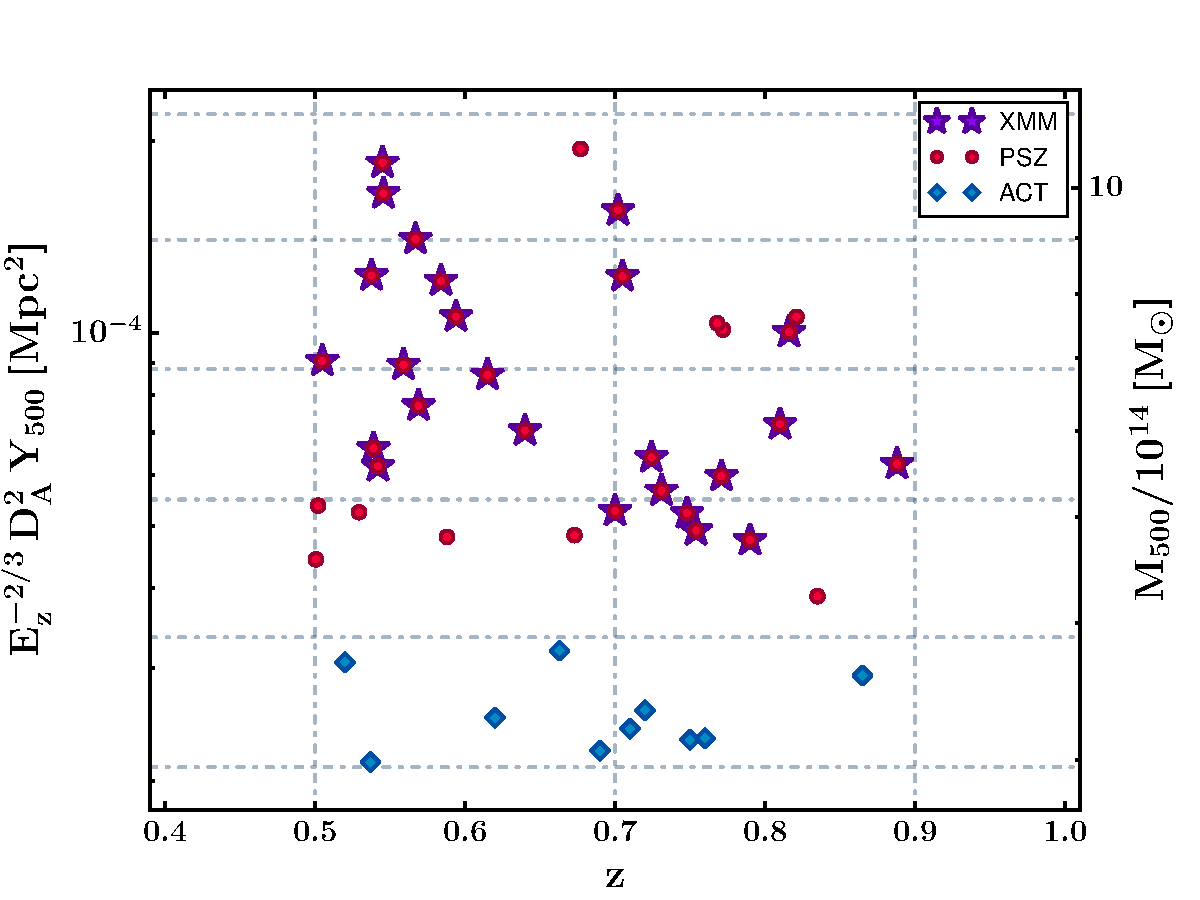
\includegraphics[width=0.44\textwidth, clip=true, trim=0cm -0.7cm 0cm 0cm]{Figures/NIKA2-SZ/LPSZ_M_z_grid.pdf}
  \caption{Left: Map of the kinetic SZ effect toward \mbox{MACS~J0717.5+3745} using NIKA pathfinder data, as discussed in Adam et al. (2017)$^{31}$. Right: NIKA2 Guaranteed-time cosmology program sample of galaxy clusters}
  \label{fig:LP-SZ}
\end{figure}
%
L'échantillon se distribue dans
deux intervalles de redshifts, les redshifts intermédiaires dans la
gamme 0.5 à 0.7 et les hauts redshifts entre 0.7 et 0.9. Il se découpe
en cinq intervalles en masse, définis à partir de la quantité
$E_{z}^{-2/3} D_{\rm{A}}^2 Y_{500}$ fortement corrélée à la masse. Cette
quantité dépend de l'observable tSZ intégré $Y_{500}$ et du modèle
cosmologique à travers $E_{z} = H(z)/H_0$ et $D_{\rm{A}}$, la distance
angulaire. Nous avons sélectionné cinq amas cibles dans chacun des
intervalles en redshift et en masse en utilisant des critères assurant
la représentativité de l'échantillon. Cette propriété est fondamentale
pour fournir des mesures des relations d'échelle et des profils
thermodynamiques applicables à l'ensemble des amas et donc utiles pour
les analyses cosmologiques. Comme discuté à la Sect.~\ref{se:cosmo_sz}, une
sélection basée sur le signal tSZ capture presque tous les amas
au-dessus d'un seuil en masse, et définit bien un échantillon
représentatif. Ainsi, les amas du LP-SZ sélectionnés sont ceux
appartenant à un catalogue d'amas détectés via le tSZ, dont le
redshift est dans la gamme 0.5-0.9 et qui sont observables depuis le
télescope de 30-m de l'IRAM. Pour ce dernier critère, nous retenons
les amas dont la déclinaison est $\delta > -11^{\circ}$, comme figuré
par le cercle pointillé sur le panneau de gauche de la
Fig.~\ref{fig:LP-SZ}. Les quatre intervalles de plus hautes masses sont
peuplés par des amas sélectionnés dans le premier catalogue de
\emph{Planck}~\citep[le seul disponible au moment de la définition de
l'échantillon][]{Planck2013_SZcat}, tandis que les amas de
l'intervalle de basse masse sont issus du catalogue
ACT~\citep{Hasselfield2013_ACT_SZ}.

Par ailleurs, les observations tSZ avec NIKA2 seront complétées par
des suivis avec d'autres sondes. En particulier, la complémentarité
avec les observations dans le domaine X avec le satellite
\emph{XMM-Newton} est l'une des forces du LP-SZ. Les amas du LP-SZ
également observés par \emph{XMM-Newton} sont repérés avec une étoile
dans le panneau de droite de la Fig.~\ref{fig:LP-SZ}. Des demandes de
suivi avec \emph{XMM-Newton}, portées par l'équipe du LP-SZ, sont en
cours.   

\subsection{Objectifs et livrables}

L'objectif premier du LP-SZ est de fournir à la communauté des cartes
à haute résolution angulaire de l'effet tSZ, ainsi que les profils de
pression reconstruits, pour un échantillon représentatif d'amas de
galaxies. Ces données permettront une étude approfondie des propriétés
des amas de galaxie jusqu'à haut redshift et de leur évolution
cosmologique. De même qu'un profil de pression universel a été mesuré
avec \emph{REXCESS}, un échantillon représentatif de 33 amas observés
avec \emph{XMM-Newton} dans l'univers proche
($z<0.2$)~\citep{Arnaud2010}, l'échantillon du LP-SZ permettra de
tester la régularité du profil de pression jusqu'à $z=0.9$ à partir
d'une observable sondant directement la pression. Aussi, l'impact des
sous-structures et de la morphologie des amas sur l'observable $Y_{500}$
pourra être quantifié. Des indicateurs de l'état dynamique des amas
pourront être défini à partir des observations tSZ. Ainsi, le LP-SZ
permettra de caractériser l'impact des déviations au
comportement auto-similaire sur le biais et la dispersion intrinsèque
de la relation d'échelle et du profil de pression moyen, et leur
évolution en redshift. Ces résultats attendus auront d'importantes retombées
pour la cosmologie avec les amas de galaxies.

Les objectifs scientifiques peuvent encore être étendus en exploitant
la complémentarité avec d'autres sondes des amas, et en premier lieu,
les observations dans le domaine des X. Gràce à l'expérience NIKA2, le
milieu intra-amas sera cartographié via l'effet tSZ avec le même
niveau de précision qu'en X, tant en résolution angulaire qu'en
sensibilité. Ainsi, une étude conjointe des données tSZ de NIKA2 et
des données X de \emph{XMM-Newton} permettra une caratérisation
complète des propriétés thermodynamiques des amas. Aux profils de
pression électronique $P_e(r)$ reconstruits dans les données tSZ, nous
adjoindrons les profils de densités $n_e(r)$ estimés dans les données
X. Une telle étude multi-sonde nous permettra de mesurer le profil de
température $k_{\rm{B}} T_e(r) = P_e(r)/n_e(r)$, sans avoir recourt
aux mesures spectroscopiques en X, ainsi que le profil
d'entropie $K(r) = P_e(r)/n_e(r)^{5/3}$, un bon indicateur de l'état
dynamique des amas. Ensuite, sous l'hypothèse de l'équilibre
hydrostatique, nous reconstruirons le profil de masse hydrostatique
des amas $M_{\rm{HE}} (r) \propto r^2/n_e(r) dP_e(r)/dr$.  
%\begin{equation}
%  M_{\rm{HE}} (r) = - \frac{r^2}{\mu_{\rm{gaz}}m_pn_e(r)}
%\end{equation}
L'étude statistique de ces profils thermodynamiques sera essentielle
pour caractériser les propriétés physique des amas, leur évolution en
redshift et la relation entre l'observable tSZ et la masse des amas.  


\subsection{L'équipe}
Le LP-SZ mobilise une équipe d'une vingtaine de chercheurs fortement
impliqués, comprennant des experts de l'effet SZ, qui ont joué un rôle
majeurs dans l'analyse des amas de galaxies dans \emph{Planck} et ont
mené des études tSZ à partir des observations de NIKA, des experts de
renommée mondiale des amas de galaxies observés en X, des experts de
simulations hydrodynamiques et des experts d'autres sondes d'amas
(observations optiques et radio). Par ailleurs, plusieurs membres ont
une connaissance très fine de l'instrument NIKA2. En tant que co-PI,
je coordonne les activités conjointement avec le PI.



%----------------------------------------------------------------------------------------
%
%
%
%
%
%                 ETUDES PILOTES ET Premiers resultats 
%
%
%
%----------------------------------------------------------------------------------------
\section{Les études pilotes et les premiers résultats}
\label{se:NIKANIKA2_SZ}

\subsection{\'Etudes pilotes avec le prototype NIKA}
\label{se:NIKA_SZ}

Pour démontrer les capacités de NIKA2 pour la cartographie
haute-résolution de l'effet tSZ, valider et optimiser la définition
des objectifs scientifiques et préparer l'analyse, nous avons d'abord
réalisé une séries d'études ``pilotes'' avec l'instrument précurseur
NIKA. Ainsi, la première détection de l'effet tSZ jamais obtenue avec
la technologie KID a été réalisée avec les observations de NIKA vers
l'amas RX\,J1347.5-1145, un amas massif à redshift intermédiaire
($z = 0.45$)~\citep{Adam2014}. Ensuite, pour préparer l'analyse tSZ de
NIKA2, des méthodes novatrices ont été développées et testées sur les
observations de NIKA. Par exemple, nous avons développé une analyse
multi-sonde combinant données tSZ et données X qui a été testée sur un
amas à haut redshift ($z = 0.89$), CL\,J1226.9+3332, observé avec NIKA
et appartenant au catalogue de données publiques de
\emph{CHANDRA}~\citep{Adam2015}. Aussi, en ciblant un amas bien régulier,
MACS\,J1423.9+2404, nous avons caractérisé l'impact des sources
ponctuelles radio et infrarouge et proposé une méthode pour les
traiter dans le cadre d'une analyse tSZ~\citep{Adam2016}. Une méthode
non-paramétrique pour reconstruire le profile de pression à partir de
la carte tSZ a été proposée et validée avec les données de NIKA et
\emph{Planck} seules~\citep{Ruppin2017} et en considérant aussi les
données de MUSTANG et BOLOCAM~\citep{Romero2018}. Nous avons exploré
la présence de sous-structures dans le milieu intra-amas, signant
l'état dynamique de l'amas, en testant plusieurs outils de détection
dans les cartes tSZ de NIKA~\citep{Adam2018_sub}. Cette étude, qui a
accompagnée la livraison des données tSZ de NIKA à la communauté,
constitue une validation de la possibilité pour NIKA2 de caractériser
l'impact de l'état dynamique des amas sur le profil de pression moyen
et la relation masse-observable tSZ.

%
\begin{figure}
  \centering
  \includegraphics[width=0.40\textwidth]{Figures/NIKA2-SZ/MACSJ0717_T_map.pdf}
  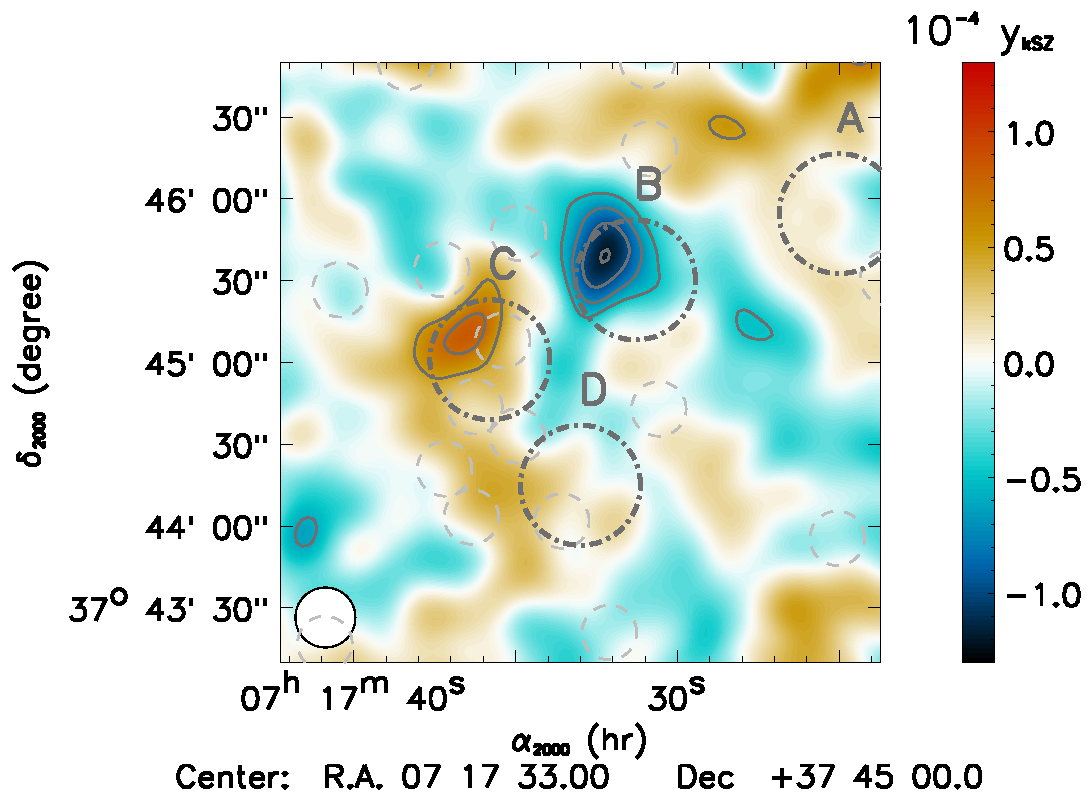
\includegraphics[width=0.56\textwidth]{Figures/NIKA2-SZ/MACSJ0717_kSZ_map.pdf}
  \caption{Map of the kinetic SZ effect toward \mbox{MACS~J0717.5+3745} using NIKA pathfinder data, as discussed in Adam et al. (2017)$^{31}$.}
  \label{fig:nikanika2}
\end{figure}
%
Ces études pilotes nous ont aussi permis d'obtenir des résultats
remarquables, allant au-délà de ce qui étaient initialement espéré, et
marquant une percée vers des études novatrices. En particulier,
la première carte de la température du milieu intra-amas reconstruite
avec l'effet SZ est décrite dans~\citet{Adam2017} et la première carte
de l'effet SZ cinétique (kSZ) mesuré dans un amas a été obtenue 
dans~\citet{Adam2017kSZ}. Ici nous présentons brièvement ces deux
résultats.

La température du milieu intra-amas est une observable fondamentale pour
caractériser les amas de galaxies, en particulier pour déterminer leur
masse hydrostatique. Cette température est généralement obtenue par
mesures spectrométriques dans le domaine X. Cette méthode a plusieurs
limitations bien connues. L'émission X étant proportionnelle au carré
de la densité du milieu intra-amas, les mesures en X sélectionnent
préférentiellement les zones denses et froides des amas. Ensuite, les
mesures de température via les expériences X actuels, tels
\emph{XMM-Newton} et \emph{Chandra}, sont affectées par l'incertitude
sur la calibration absolue en énergie, qui est de l'ordre de
$15\%$. Enfin, une mesure précise de la température par spectroscopie
X requiert de longs temps d'observation, qui peuvent même devenir
prohibitifs pour les amas distants. Une autre méthode pour obtenir la
température du milieu intra-amas consiste à la reconstruire à partir
de la pression électronique mesurée via l'effet tSZ et de la densité
mesurée par photométrie X, par exemple. En utilisant cette méthode,
\citet{Adam2017} a construit la première carte de la température d'un
amas, MACS\,J0717.5+3745, en combinant les observations SZ
haute-résolution de NIKA et les données photométriques de
\emph{XMM-Newton}. Cette carte, présentée dans le panneau de gauche de
la figure~\ref{fig:nikanika2}, met en évidence un fort gradient de
température dans la région de collision entre les deux principaux
sous-amas. Elle est compatible avec les cartes de température dérivées
des données spectroscopiques de \emph{XMM-Newton} et \emph{Chandra},
tout en étant moins bruitées et obtenue avec un temps d'observation
trois fois moindre.


L'effet kSZ est dù au mouvement d'ensemble du milieu intra-amas, il
dépend à la fois de la densité du gaz et de sa vitesse propre par
rapport au référentiel du CMB et, contrairement au tSZ, ne crée pas de
distortion spectrale (voir discussion Sect.~\ref{se:cosmo_sz}). Par
conséquent, sa signature en fréquence diffère de celle du tSZ. En
combinant des cartes dans différent canaux de fréquence du domaine
millimétrique, les deux composantes peuvent être séparées, et une
carte reconstruite pour chacune d'entre elle. En pratique, une telle
étude requiert une expérience qui allie une haute sensibilité, afin de
détecter cet effet sous-dominant, et une grande résolution angulaire
afin de séparer spatialement le kSZ du CMB. Le panneau de droite de la
figure~\ref{fig:nikanika2} présente la première carte résolue
du kSZ, obtenue par~\citet{Adam2017kSZ} en combinant les
observations à 150 et 260\,GHz effectuées avec NIKA vers l'amas
MACS\,J0717.5+3745. Cet amas bien connu, déjà choisi comme
cible pour cartographier la température, est un système complexe, très
perturbé, composé de plusieurs sous-amas en interaction, avec des
vitesses relatives extrêmes (de l'ordre de 1000\,km/s). Ces sous-amas
sont entourés en gris sur la figure~\ref{fig:nikanika2}, deux d'entre
eux tombent l'un vers l'autres et induisent un effet kSZ de signe
opposé. En combinant les cartes de NIKA avec une mesure de la
température du gaz issue des données spectroscopiques de
\emph{XMM-Newton}, les cartes de densité et de vitesse du gaz ont été
reconstruites en supposant un modèle de gaz. Ainsi a été obtenue la
première carte résolue de la vitesse au sein du milieu intra-amas
mesurée via l'effet kSZ.

Ces résultats nous donnent une grande confiance dans notre capacité à
réaliser les objectifs scientifiques que nous nous somme fixés dans le
cadre du LP-SZ et au-delà, de l'utilité pour la cosmologie des
observations CMB à très haute résolution.

\subsection{Premiers résultats de NIKA2}

Les observations des amas de galaxies du LP-SZ ont d'ores et déjà
commencées. La première observation d'un amas a été
effectuée dès la phase de vérification scientifique de NIKA2 en avril
2017 (voir l'historique à la Sect.~\ref{}), puis les observations se
sont poursuivies depuis l'ouverture de NIKA2 à la communauté en
octobre 2017, de sorte que 19 amas du LP-SZ ont été observés pour un
temps d'observation total d'environ 80 heures.


Pour la vérification scientifique, nous avons sélectionné un amas du
LP-SZ avec un fort signal tSZ attendu et pour lequel nous disposions
aussi de données X à haute précision. Ainsi, le premier amas observé
du LP-SZ est PSZ2\,G0144.83+25.11, un amas bien connu, massif
($\rm{M} = 7.8\,10^{14}\,\rm{M}_{cdot}$), à redshift intermédiaire
($z=0.58$) et observé également par \emph{XMM-Newton}. Les données
NIKA2 consistent en 11 heures d'intégration sur la source, soit cinq
fois plus que le temps demandé dans le LP-SZ pour cet amas, mais dans
des conditions de forte attenuation atmosphérique (opacité de 0.3 à
150\,GHz). Après soustraction des sources ponctuelles par une méthode
adaptée de celle de~\citet{Adam2016}, nous avons
obtenu la première carte du paramètre de Compton vers un amas de
galaxie avec NIKA2. Cette carte, décrite dans~\citet{Ruppin2018}, est
présentée dans le panneau de gauche de la figure~\ref{fig:nika2-sz}.
%
\begin{figure}
  \centering
  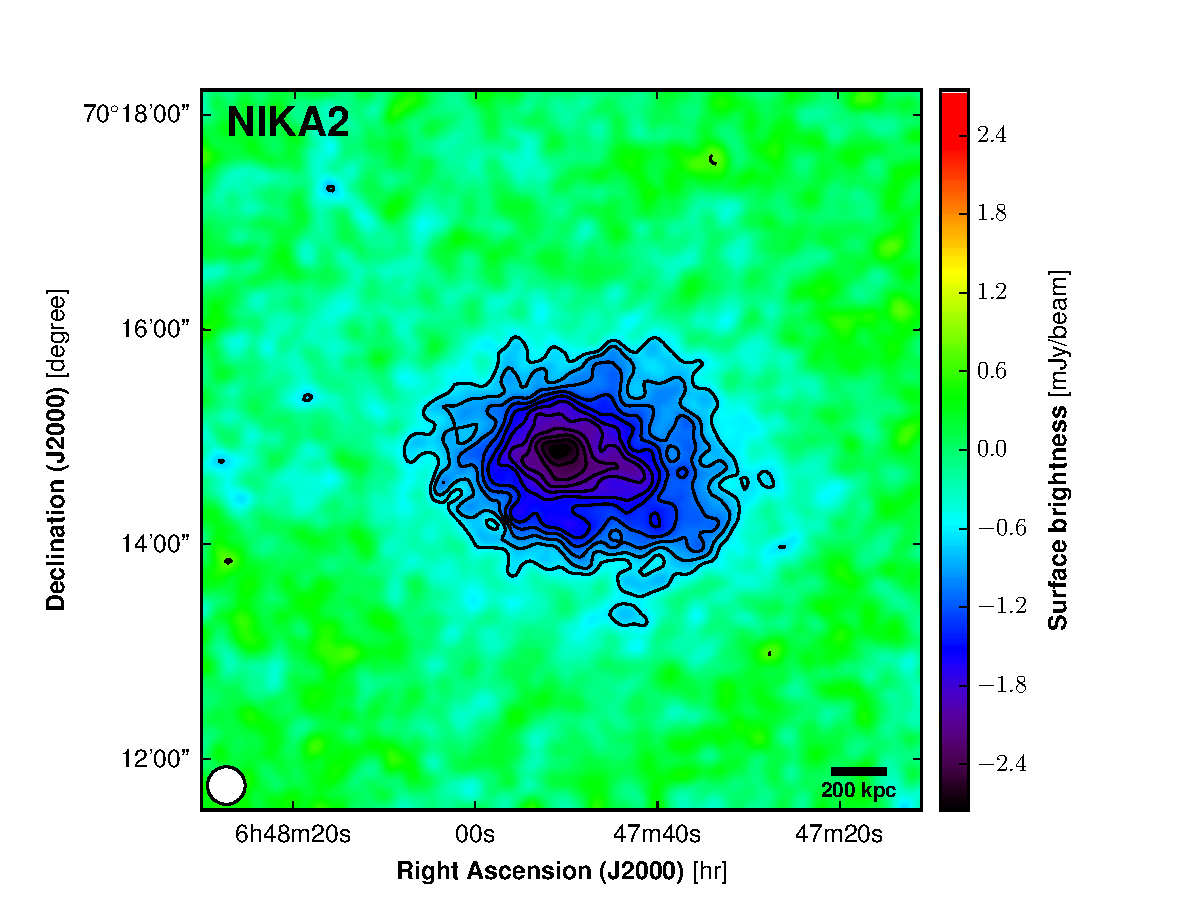
\includegraphics[width=0.49\textwidth]{Figures/NIKA2-SZ/Paper_NIKA2_Data.pdf}
  \includegraphics[width=0.44\textwidth]{Figures/NIKA2-SZ/Fig_PSZ2_G144_Scaling_relation.pdf}
  \caption{First SZ results with NIKA2. Left: The NIKA2 SZ map toward the galaxy cluster PSZ2-G0144.83+25.11. The high-resolution (20~arcsec) high-accuracy ($13.5\sigma $ measurement at peak) map covers the cluster from the core to the outskirts and reveals its morphology. An excess SZ signal is observed in the South-West region, indicating an overpressure within the intracluster medium (ICM). Right: Illustration of the impact of the ICM dynamics on the inner scatter of the SZ mass-observable relation. NIKA2 $Y_{500}$ estimates from the analysis with and without masking the over-pressure of PSZ2-G0144.83+25.11 are shown as a function of $M_{500}$, along with the cluster sample and the $Y_{500}-M_{500}$ scaling relation used in \emph{Planck} SZ-selected cluster count based cosmology analysis$^{13}$. These figures are extracted from Ruppin {\it et al.} (2018)$^{34}$. }
  \label{fig:nika2-sz}
\end{figure}
%
Nous avons identifié une zone de sur-pression thermique dans l'extension sud-ouest
de l'amas, qui est repérée par la zone grisée sur la
figure~\ref{fig:nika2-sz}. Pour cet amas, en plus des cartes tSZ de
NIKA2 et \emph{Planck}, nous disposons de la carte tSZ de MUSTANG, dont
la résolution angulaire est de 9'' et le champ de vue de
42''~\citep{Young2015}, ainsi que de celle de BOLOCAM, sur un champ de
vue de 8' pour une résolution angulaire de l'ordre de
1'~\citep{Sayers2013}. Tout d'abord, en combinant l'ensemble des
données tSZ, nous avons obtenue une mesure non-paramétrique du profil
de pression depuis le coeur de l'amas ($\sim 0.02\rm{R}_{500}$)
jusqu'à sa périphérie ($\sim 3\rm{R}_{500}$) en utilisant la méthode
développée dans~\citet{Ruppin2017}. Ensuite, nous avons exploré
l'impact de la sur-pression en comparant les profils de pression
reconstruits soit dans les cartes tSZ de NIKA2 et \emph{Planck}
complètes, soit en masquant la sur-pression. Nous observons une
différence significative entre les deux profils résultants. Le profil
déprojetté sur les cartes masquées est en accord avec le profil de
pression universel décrit dans~\citet{Arnaud2010}, mais dévie
significativement du profil obtenu dasn les cartes non-masquées, ce
dernier étant en accord avec le profil publié dans~\citet{Young2015} à
partir des cartes tSZ complètes de MUSTANG et BOLOCAM. 
Pour aller plus loin, nous avons réalisée une analyse conjointe des
données tSZ de NIKA2 et \emph{Planck} et des données X de
\emph{XMM-Newton}, en utilisant une méthode adaptée
de~\citet{Adam2015}, pour dériver les profils thermodynamiques de
l'amas sous l'hypothèse d'équilibre hydrostatique. Nous trouvons que
le paramètre de Compton intégré jusqu'à $R_{500}$, $\rm{Y}_{500}$ et
la masse hydrostatique $\rm{M}_{500}$ résultant des analyses
hydrostatiques effectuées avec ou sans le masque de la zone de
sur-pression diffèrent significativement. Ces valeurs sont reportées
dans le panneau de droite de la figure~\ref{fig:nika2-sz}, et
superposées aux quantités intégrées pour l'échantillon d'amas de
\emph{Planck} qui a servi à calibrer la relation d'échelle utilisée
pour les résultats
cosmologiques~\citet{Planck_2014_SZ_Cosmo,Planck_2016_SZ_cosmo}. Cette
étude est une indication de l'impact de l'état thermodynamique des
amas sur la dispersion intrinsèque de la relation
masse-observable. Elle illustre bien l'utilité de NIKA2, combinée avec
des données X, pour caractériser la relation d'échelle.   






%----------------------------------------------------------------------------------------
%
%
%
%
%
%                 Prospectives ? 
%
%
%
%----------------------------------------------------------------------------------------
\section{Développement de l'analyse, implication pour la cosmologie et perspectives}

\subsection{Préparation de l'analyse cosmologique}

\`A court terme, l'équipe du LP-SZ s'attachera à préparer l'analyse, la
publication et la livraison à la communauté scientifique des données
et résultats d'intérêt cosmologique.

\subsubsection{Vers une méthode standard d'analyse}
La première étape consistera en 1)
l'amélioration et 2) la standardisation des outils d'analyse. Les
améliorations viseront en priorité le traitement des sources
ponctuelles, qui constituent le contaminant majeur des cartes tSZ de
NIKA2. Une telle étude, centrée sur l'optimisation du traitement des
sources ponctuelles infrarouge pour les amas les moins brillants de
l'échantillon du LP-SZ, est déjà en cours~\citep{Keruzore2020}.

Un deuxième champ d'amélioration crucial concerne la reconstruction
des grandes échelles angulaires. En effet, tandis que les observations en X
révèlent bien les zones centrales (denses et froides) de l'amas, les
observations tSZ permettent une cartographie s'étendant sur de grandes
distances jusque dans la périphérie de l'amas. Pour exploiter au mieux
cette caractéristique et bénéficier du grand champ de vue de NIKA2, il
nous faut développer des outils d'analyse qui préservent les grandes
échelles angulaires. Or nos méthodes actuelles sont efficaces pour
soustraire le bruit corrélé issu majoritairement de l'émission
atmosphérique, au prix d'un filtrage spatial~\citep[voir par
  exemple][]{Ruppin2018}. Des pistes de développement de nouvelles
méthodes sont actuellement explorées.

Quant à la standardisation des outils d'analyse, elle est nécessaire
afin de ne pas briser la représentativité de l'échantillon d'amas du
LP-SZ en introduisant des biais méthodologiques. Il nous faudra
développer des outils robustes, applicables pour toutes les
morphologies d'amas et pour toutes la gamme de signal tSZ sondé. Ces
méthodes seront testées et optimisées sur des simulations.

\subsubsection{Validation et études prospectives}

La validation des outils d'analyse sur simulation est un volet
important du LP-SZ. Nous déployons à la fois des simulations simples,
utilisant un profil de pression universel pour synthétiser un signal
tSZ, permettant une analyse Monte-Carlo, et à la fois des simulations
réalistes. Ces dernières sont basées sur la simulation hydrodynamique
\emph{Marenostrum MUltidark SImulations of galaxy
  Clusters}~\citep[MUSIC][]{Sembolini2013}. Ainsi, un échantillon
d'amas synthétiques a été extrait de la simulation MUSIC de façon à
obtenir un échantillon similaire à celui du LP-SZ. Cet échantillon
``jumeau", qui présente le même peuplement dans le plan
masse-redshift, est décrit dans~\citet{Ruppin2019a}. Il a été utilisé
pour tester nos outils de reconstruction du profil de pression dans le
milieu intra-amas. Pour cela, des observations réalistes des amas
synthétiques par NIKA2 et \emph{Planck} ont été simulées, et les
profils de pression estimés sur ces simulations. La comparaison entre
les profils de pression moyens reconstruits et simulés nous permet de
valider les méthodes de reconstruction. \citet{Ruppin2019a} ont montré
que le profil de pression moyen était bien reconstruit, avec une
précision de l'ordre du pourcent, quelque soit l'état dynamique de
l'amas. En plus du test des méthodes d'analyse, cette étude a mis en
évidence l'impact sur le profil de pression moyen de l'état dynamique
des amas. En effet, la dispersion intrinsèque du profil de pression
moyen est sensiblement plus grande pour les amas perturbés, présentant
des sous-structures, que pour les amas réguliers, à l'équilibre
hydrostatique. Bien que la forme et la dispersion du profil moyen
dépendent de l'échantillon synthètique, cette étude prospective est
bien représentative des résultats qui pourront être obtenus dans le
cadre du LP-SZ. D'autres études prospectives pourront être menées en
exploitant les simulations MUSIC, incluant l'optimisation de critères
dichotomiques de l'état thermodynamique des amas
(réguliers/perturbés) ou la caractérisation de l'impact d'une déviation
à l'auto-similarité sur le profil de pression moyen et la relation
masse-observable.

\subsubsection{Préparation de la livraison des données et des résultats}

Nous nous attacherons à préparer la livraison des données à la
communauté, et la publication des résultats d'intérêt cosmologique,
qui devront avoir lieu entre 2022 et 2025. En plus des cartes tSZ à hautes
résolution angulaire de NIKA2, nous publierons notre caractérisation
du profil de pression universel et de la relation masse-observable,
et dériverons les implications pour la cosmologie. 
%
\begin{figure}
  \centering
  \includegraphics[width=0.49\textwidth]{Figures/NIKA2-SZ/NIKA2cosmo_echantillon_calibration.pdf}
  \includegraphics[width=0.49\textwidth]{Figures/NIKA2-SZ/NIKA2cosmo_param.pdf}
  \caption{Left: Distribution of the 62 Planck clusters used to
    estimate the mean normalized pressure profile at low redshift
    (purple) in the mass-redshift plane. The NIKA2 and REXCESS samples
    are also shown in orange and green respectively.
    The different shades of blue give the expected cluster abundance,
i.e. the cluster number per unit of mass and redshift. Right:
Constraints obtained on the $\sigma_8$ and $\Omega_m$ cosmological
parameters using the Pm profile (grey) and the Pm profile scaled down
by 15\% (green) for a possible future hydrostatic bias prior of $b = 0.20
\pm 0.01$. The constraints obtained from the joint analysis of the CMB
primary anisotropies and BAO data are also shown in purple. Figures
from~\citet{Ruppin2019b}}
  \label{fig:nika2cosmo}
\end{figure}
%
Le LP-SZ résultera en une amélioration de la calibration de la masse des
amas de galaxies et de leur contenu thermodynamique par rapport à
notre connaissance actuelle. Ce potentiel d'amélioration est illustré
dans le panneau de gauche de la
figure~\ref{fig:nika2cosmo}. L'échantillon d'amas du LP-SZ est comparé
aux échantillons d'amas qui fondent actuellement la calibration des
amas de galaxies dans les analyses cosmologiques de
\emph{Planck}~\citep{Planck_2014_SZ_Cosmo,
  Planck_2014_ymap, Planck_2016_SZ_cosmo, Planck2016_ymap,
  Salvati2018}. Dans le plan mass-redshift, sont figurés l'échantillon
de 45 amas du LP-SZ, qui couvre l'intervalle $0.5 \le z \le 0.9$,
l'échantillon de 62 amas de \emph{Planck} à $z<0.5$ sur lequel est
calibré le profil de pression moyen, et l'échantillon de 31 amas de
REXCESS~\citep{Pratt2009} qui a servi à calibrer la relation
masse-observable et le profil de pression universel via les
observations en X, comme décrit dans \citet{Arnaud2010}. En sondant un
échantillon d'amas distants,
le LP-SZ permettra de contraindre l'évolution en redshift des
propriétés des amas et fournira des mesures de la relation
masse-observable et du profil de pression moyen bien adaptées aux
relevé d'amas cosmologiques. En améliorant la calibration des amas de
galaxies, qui constitue la limitation principale des études
cosmologiques, nous améliorerons la robustesse et la précision des
contraintes cosmologiques dérivées des amas de galaxies.

Dans des études prospectives, nous pouvons déjà prédire l'impact des
résultats du LP-SZ sur la cosmologie. Par exemple, \citet{Ruppin2019b}
ont étudié l'impact du profil de pression moyen sur les contraintes
cosmologiques dérivées du spectre de puissance angulaire de l'effet
tSZ de \emph{Planck}. Dans le cadre du modèle $\Lambda$CDM standard,
nous avons trouvé des différences signicatives sur les paramètres
cosmologiques estimés en fonction du  profil de pression moyen supposé
dans l'analyse cosmologique. Dans le panneau droit de la
figure~\ref{fig:nika2cosmo}, nous traçons les contours à 68 et 95\% de
niveau de confiance de la distribution de paramètres dans le plan
$\sigma_8$, $\Omega_{\rm{m}}$ pour trois analyses cosmologiques :
une analyse conjointe du CMB de
\emph{Planck}~\citep{Planck_2018_cosmo} et des oscillations
acoustiques des baryons (BAO) de BOSS~\citet{Anderson2014}, l'analyse
du $C_\ell^{\rm{tSZ}}$ de \emph{Planck} en supposant le même profil de
pression moyen que celui utilisé dans \citet{Planck2016_ymap} et la
même analyse réitérée avec un profil de pression moyen d'une amplitude
15\% inférieure. Nous concluons qu'une diminution de 15\% de
l'amplitude du profil de pression moyen suffit pour pour faire
coïncider les modèles cosmologiques favorisés par le CMB primaire et
par les amas de galaxies sans avoir recours à des valeurs extrêmes du
biais hydrostatique. L'apport du LP-SZ sur la mesure du profil de
pression moyen et son évolution en redshift sera donc précieux pour
contraindre la cosmologie avec les amas de galaxies. 

D'autres études prospectives pourront être menées pour anticiper la
livraison des résultats du LP-SZ. Par exemple, une évolution de la
forme ou la dispersion intrinsèque de la relation masse-observable
pourrait biaiser l'estimation de la fonction de sélection de
l'échantillon cosmologique dans le cadre d'une analyse fondée
sur le comptage des amas, et aurait ainsi un impact important sur le
modèle cosmologique estimé. Ou encore, une étude similaire à
celle menée dans~\citet{Ruppin2019b} pourrait être conduite dans le
cadre d'un modèle cosmologique étendu en utilisant les outils
développés dans~\citet{Bolliet2018, Bolliet2019} pour étudier l'impact
de la calibration des amas de galaxies sur les contraintes de
l'énergie noire ou la masse des neutrinos.\\

Le travail décrit dans cette section, et qui aboutira à la
publication des résultats du LP-SZ pourrait faire l'objet d'une thèse
de doctorat commençant au début de la décennie 2020. 

\subsection{\'Etudes multi-sondes complémentaires}

Au delà de l'analyse principale centrée sur la combinaison des données
X et tSZ, décrite à la section précédente, des analyses multi-sondes
complémentaires pourraient encore enrichir les résultats du LP-SZ. 

\subsubsection{Relation entre milieu intra-amas et galaxies avec les
  données optiques}

Des données de haute qualité en imagerie et en spectroscopie optique
et proche infrarouge, utilisées en combinaison avec le tSZ et le X,
conduiraient à plusieurs développements importants. Nous disposerions
alors à la fois des mesures de la richesse, c'est-à-dire le nombre de
galaxies membres, et des mesures de leur dispersion de vitesse, nous
fournissant chacunes une estimation supplémentaire de la masse des
amas, fondées sur des hypothèses différentes de la masse hydrostatique
tSZ-X et non affectées par les même effets systématiques. De telles
études combinées nous permettraient d'explorer les correlations entre
la richesse, la masse dynamique, calculée à partir de la dispersion de
vitesses, et la masse hydrostatique et plus généralement la relation
entre les propriétés des galaxies au sein des amas et le milieu
intra-amas.

Pour ce programme, nous avons envisagé d'effectuer un suivi des amas
du LP-SZ avec les imageurs et spectromètres installés au \emph{Gran
  Telescopio Canarias} (GTC), le télescope de 10.4 mètres de
l'\emph{Instituto de Astrofísica de Canarias} (IAC), situé sur l'île
de La Palma. Ce télescope est bien adapté pour le suivi optique des
amas \emph{Planck} distants et visibles depuis l'hémisphère
nord. Un tel suivi est actuellement en cours dasn le cadre des grands
programmes d'observation optique visant à la validation et la
caractérisation des catalogues d'amas de
\emph{Planck}~\citep{Barrena2018,Streblyanska2019,Aguado-Barahona2019}.
Pour le suivi des amas du LP-SZ, des observations plus profondes
seront nécéssaires afin de caractériser la structure interne des
amas. Quelques heures d'observation par amas avec la caméra OSIRIS du
GTC permettraient d'effectuer à la fois une photométrie dans les
filtres \emph{GRIZ} et une spectroscopie multi-objets avec un rapport
signal-sur-bruit suffisant pour caractériser la distribution des
galaxies membres dans l'espace des phases. Des études multi-sondes
combinant les données tSZ, X et optique donneraient de précieuses
indications sur l'interaction des populations de galaxies avec le
milieu inter-amas. Ensuite, un suivi en spectro-imagerie optique de
l'échantillon du LP-SZ permettrait d'une part de contraindre la
relation entre masse dynamique et la masse hydrostatique et son
évolution en redshift, et d'autre part de mieux comprendre la
formation et l'évolution des populations de galaxies dans les amas.
Une telle étude, complémentaire aux objectifs c\oe ur du LP-SZ,
auraient d'importantes implications pour la cosmologie avec les amas
de galaxies, en particulier dans le cadre de futurs relevés optiques
(Euclid, LSST). 


\subsubsection{Contraindre le biais hydrostatique et la pression
  non-thermique avec l'effet de lentille}

Les effets de lentille fort et faible sur les galaxies d'arrière-plan
dépendent du potentiel gravitationnel de l'amas intégré le long de la
ligne de visée, et permettent ainsi une reconstruction de la masse
totale de l'amas. Les effets systématiques qui impactent cette mesure
sont de nature instrumentale (incertitude sur la PSF), méthodologique
(calibration du cisaillement, contamination par des galaxies
d'avant-plan) ou géométrique (alignement, tri-axialité, décentrage),
mais ne dépendent pas de l'état thermodynamique de l'amas. Ainsi, des
analyses conjointes du tSZ, des X et des lentilles
permettent à la fois de mieux contraindre la masse des amas, et à la
fois de tester les hypothèses qui fondent l'estimation de la masse à
partir de chacune de ces observables. Comme mentionné dans la
Sect.~\ref{se:cosmo_tensions}, de telles analyses, utilisant les
programmes de reconstrution de l'effet de lentille récents (Weighting
the Giants, CCCP, LoCuSS), ont permis de mesurer le biais
hydrostatique~\citep[voir][pour une compilation des
  résultats]{Salvati2018, Osato2019}. Autre exemple pris dans la littérature
récente, \citet{Siegel2018} ont combiné le tSZ mesuré par BOLOCAM, les
données X de \emph{Chandra} et les effets de lentilles mesurés avec le
\emph{Hubble Space Telescope} (HST) et \emph{Subaru Suprime-Cam}. En
comparant le profil de pression thermique estimé dans les données
tSZ-X et le profil de pression totale nécessaire pour empêcher
l'effondrement gravitationel, ils ont déduit une mesure de la pression
non-thermique, induite par la turbulence ou les écoulements au sein du
milieu intra-amas. De la même façon, les données tSZ-X du LP-SZ,
combinées aux mesures existantes de l'effet de lentille, nous
permettront de mesurer le biais hydrostatique et la fraction de pression
non-thermique et de contraindre leur évolution en redshift.  

\subsubsection{Mesurer la pression électronique jusqu'au c\oe eur des
  amas : synergie avec NOEMA}

NIKA2 cartographiera les amas de galaxies avec une résolution angulaire
et une sensibilité comparable à celles de \emph{XMM-Newton},
permettant une exploitation optimale de la complémentarité des données
X et tSZ au sein du LP-SZ. Ce programme bénéficierait d'observations à
encore plus haute résolution angulaire pour déceler l'impact des
processus astrophysiques dans le milieu intra-amas, en particulier au
c\oe ur des amas. Pour cela, l'interférométrie millimétrique est
parfaitement adaptée puisqu'elle permet une cartographie très haute
résolution des amas distants via l'effet tSZ. Dans l'hémisphère sud,
l'interféromètre millimétrique phare est ALMA. La complémentarité des
observations tSZ à résolution angulaire de quelques secondes d'arc à
quelques minutes d'arc a été exploitée pour une mesure complète du
profil de pression d'un amas en combinant les données
interférométriques d'ALMA avec les données des imageurs BOLOCAM et
\emph{Planck}~\citep{DiMascolo2019}. Dans l'hémisphère nord, le plus
grand interféromètre millimétrique actuellement en opération est le
\emph{NOrthern Extended Millimeter Array} (NOEMA) de l'IRAM.

NOEMA\footnote{Site web :
  \url{https://www.iram-institute.org/EN/content-page-56-7-56-0-0-0.html}}
est un réseau de 10 antennes de 15 mètres de diamètres, installé
au Plateau de Bure. Il observe dans trois bandes
de fréquence centrées à 90, 150 et 230 GHz avec une résolution
angulaire allant de quelques secondes d'arc à quelques dizièmes de
secondes d'arc selon la configuration des antennes, sur un champ de
vue $\lesssim 0.5'$. Un suivi des amas du LP-SZ avec NOEMA permettrait
d'obtenir une mesure globale du profil de pression incluant le c\oe ur
des amas qui ne peut pas être cartographié par NIKA2 et
\emph{XMM-Newton}. Les observations tSZ de NOEMA affinerait notre
connaissance des chocs entre sous-halos des amas non-réguliers, des
turbulences et autres processus baryoniques dans le milieu intra-amas,
nous permettant de mieux comprendre, et \emph{in fine} de corriger,
leur impact sur la reconstruction de la masse des amas.



\subsection{Perspectives d'extensions du grand programme SZ}

Le LP-SZ bénéficie de 300 heures d'observation garantie, qui ont été
distribuées entre les 50 amas de l'échantillon cible de façon à
préserver sa représentativité. Ainsi, chaque amas est observé
suffisament longtemps pour garantir une mesure à 3$\sigma$ du profil de
pression à $R_{500}$. De telles observations sont bien adaptées aux
objectifs scientifiques principaux du LP-SZ, mais n'épuisent pas les
possibilités de cartographie des amas de galaxie avec NIKA2. En
attestent le nombre, la diversité et la qualité des observations des
amas de galaxies réalisées sur demandes de temps ouvert. Nombre
d'entre ces projets sont particulièrement enthousiasmants. Par
exemple, les observations SZ de NIKA2 servent à des études complètes
de la dynamique d'amas complexes à haut redshift, pourraient permettre
une première cartographie de la température via l'effet SZ
relativiste, ainsi que la cartographie de la vitesse des amas via
l'effet SZ cinétique. Plusieurs extensions au LP-SZ, avec de fortes
implications pour la cosmologie avec les amas de galaxies, pourraient
être envisagées, incluant des observations plus profondes, visant
davantage de cibles, à plus basses masses et/ou plus hauts redshifts. 
Parmi ces extensions possibles, je choisis d'en décrire trois qui me
motivent en ce qu'elles ouvrent chacunes de nouvelles pistes de
recherche prometteuses pour la cosmologie.


\subsubsection{Détection de l'effet de lentille d'un amas sur le CMB}

En plus de la diffusion par le milieu intra-amas, le CMB est perturbé
par l'effet gravitationnel des amas de galaxies. Ainsi, les photons du
CMB voient leur tragectoire légèrement défléchie à la traversée du
potentiel gravitationel d'un amas de galaxie. Cet effet de lentille
gravitationnelle des amas sur le CMB dépend du potentiel gravitationel
intégré le long de la ligne de visée, imprime sa signature dans les
cartes des anisotropies de température et de polarisation du CMB, et
peut être utilisé pour reconstruire la masse de
l'amas~\citep{Seljak2000, Hu2007}.

Cet effet a été récemment détecté dans les données de
ACTPol~\citep{Madhavacheril2015} et SPT~\citep{Baxter2015} par
accumulation des mesures aux positions indiquées dans les catalogues
d'amas. \citet{Melin2015} ont proposé l'utilisation d'une telle méthode
cumulative pour calibrer la masse des amas détectés via le
tSZ  dans les expériences CMB actuelles~\citep{Melin2015}. Cette
calibration a été réalisée pour les données tSZ de
\emph{Planck}~\citep{Planck_2016_SZ_cosmo, Zulbedia2019}. 
Cette technique, qui constitue une calibration de la relation
masse-observable en interne, se généralisera pour l'exploitation
cosmologique des données tSZ issues des futures expériences CMB à
haute résolution angulaire, telles le \emph{simons Observatory} ou
CMB-S4~\citep{Louis2017}.

Grâce à sa résolution angulaire $\gtrsim 10'$ et son grand champ de
vue, NIKA2 pourrait obtenir la première mesure de l'effet de lentille
sur le CMB par un amas individuel, à condition que les contaminants (et
le premier d'entre eux, le tSZ) puissent être suffisament soustraits. 

\subsubsection{Détection de sources lentillées à très haut redshift}

Les amas de galaxies sont de puissantes lentilles gravitationnelles,
qui dans le régime de lentillage fort, amplifient le flux des sources
d'arrière-plan~\citep[voir \emph{e.g.} pour une
  revue][]{Kneib2011}. L'effet de lentille fort des amas de galaxie
constitue une sonde cosmologique géométrique. Il est aussi utilisé
pour reconstruire la distribution de la masse au sein des amas de
galaxies et comme "télescope cosmique'', pour observer les sources à
très hauts redshifts. Ainsi, les galaxies les plus distantes jamais
observées sont détectées via l'effet de lentille fort des
amas~\citep[voir][par exemple]{Salmon2018} Aussi,
l'effet de lentille fort offre une opportunité d'étudier les
populations des premières galaxies qui se sont
formées~\citep[voir][par exemple]{Oesch2018} et celles dites galaxies
"poussièreuses'' à flambée d'étoiles (\emph{Dusty Star Forming
  Galaxy}, DSFG). L'enjeu est de contraindre le processus de formation
des structures, de sonder l'époque de la réionisation et de mesurer
l'évolution cosmique de la formation d'étoiles. Ce projet mobilise
d'importants efforts observationnels avec le télescope \emph{Hubble},
tels les programmes \emph{Cluster Lensing And Supernova survey with
  Hubble} (CLASH), \emph{Hubble Frontier Fields} (HFF) ou le
\emph{Reionization Lensing Cluster Survey} (RELICS).

NIKA2 va détecter un nombre important de sources compactes dans
l'environnement immédiat des amas ou en leur sein. Elles comprendront
des sources radio et infrarouge; certaines situées en avant-plan de
l'amas, d'autres, des galaxies membres et d'autres encore, des sources
lentillées en arrière-plan~\citep{Adam2016, Ruppin2018}. En
exploitant la complémentarité avec les données de \emph{Herschel}, les
observations du LP-SZ pourront être utilisées pour la recherche de
sources lentillées à haut redshift~\citep{Adam2015}. Au-delà du LP-SZ,
il serait possible de réaliser un suivi des amas observés en optique
via leur effet de lentille fort (\emph{Strong Lensing}, SL), avec
NIKA2. Une telle analyse multi-sonde tSZ+SL aurait trois objectifs, i)
l'amélioration du modèle de masse de l'amas pour une meilleure
reconstruction de l'effet de lentille fort, ii) la photométrie dans le
domaine millimétrique des DSFG détectées dans l'infrarouge afin de
mieux contraindre leur SED et iii) la possibilité de détecter de
nouvelles sources lentillées à haut redshift.


\subsubsection{Calibration des futurs relévés d'amas de galaxies}

Comme évoqué à la Sect.~\ref{se:sondecosmo}, la décennie 2020 verra la
construction de catalogues de quelques $10^5$ amas de galaxies
détectés par les prochains grands relévés optique et infrarouge, tels
LSST et \emph{Euclid}, les futurs grands observatoires en X (eRosita,
Athena) et la prochaines générations d'expériences CMB
(\emph{e.~g.~}\emph{Simons Observatory}, CMB-S4). Un suivi avec NIKA2 
d'échantillons d'amas issus de ces futurs catalogues pourrait apporter
des informations critiques pour leur utilisation en cosmologie. Dans
le domaine millimétrique, il s'agirait d'observer la même sonde,
l'effet SZ, avec une plus grande résolution angulaire. Ces
observations permettraient de contraindre l'évolution de la relation
masse-observable et du profil de pression en fonction du redshift et
de la fraction d'amas non-réguliers (\emph{mergers}). Dans le domaine
X, les observations haute-résolution avec NIKA2 permettraient une
mesure de la température du milieu intra-amas des amas distants, pour
lesquels les temps d'observation nécessaires à une mesure
spectroscopique de la température deviennent rédhibitoires. 
Enfin, dans le domaine optique/IR, la cartographie haute-résolution en
tSZ d'amas à haut redshift pourrait améliorer la calibration des amas
distants pour lesquels une reconstruction de l'effet de lentille
faible ou de la dynamique des galaxies membres devient
difficile. L'apport des observations tSZ pour la calibration de la
relation entre la masse et le richesse des amas détectés par
\emph{Euclid} est détaillé plus avant au chapitre suivant. 




